\chapter[Appendix - Calculation of $\Nu$ as a function of the e-folding length $x_0$]{Supplementary materiel for Chapter~\ref{ch:chapter_plainemorte}: calculation of $\Nu$ as a function of the e-folding length $x_0$}
\label{sec:appendixA}


We derive the spatial temperature profile along the channel (Eq.~(\ref{eq:exponential_law_temperature}) and Eq.~(\ref{eq:x_0})) using the energy conservation equation
%
\begin{equation}\label{eq:energy_conservation_appendix}
\frac{\partial E}{\partial t} + \frac{\partial vE}{\partial x} = M,
\end{equation}
%
where $E = \rho_w c_w T_w S$ is the energy density of the water per unit channel length (J\,m$^{-1}$), $x$ the distance (m) along channel-flow path, $v$ the stream flow velocity (m\,s$^{-1}$), and $M$ is a source term (W\,m$^{-1}$). The source is expressed in terms of  $q$, the heat flux (Wm$^{-2}$) from the water into the ice
\begin{equation}
  M = q P_w.
\end{equation}
%
We thus assume that the only relevant heat source is negative and stems from the consumption of energy related to ice melt at the channel wall and that both heat exchange at the ice-air interface and heat production due to potential energy dissipation can be neglected. This can be justified, as these two sources are on the order of 100\,Wm$^{-1}$, which is two orders of magnitude smaller than $M$.
We write $q$ as
\begin{equation}\label{eq:heat_transfer}
q = h_t \Delta T,
\end{equation}
where $h_t$ is the convective heat transfer coefficient (the conductive heat transfer can be neglected) and $\Delta T$ is the temperature difference between water and ice. Note that since the ice temperature is 0°C, $\Delta T = T_w$.
Assuming a steady state, i.e. $\frac{\partial E}{\partial t} = 0$, using Eq.~(\ref{eq:heat_transfer}), and expressing $E$ in terms of $T_w$, the Eq.~(\ref{eq:energy_conservation_appendix}) becomes
\begin{equation}
  Q\, c_w \rho_w \frac{\partial T_w}{\partial x} = h_t T_w P_w,
\end{equation}
which uses the assumption $\frac{\partial Q}{\partial x} = 0$.  This equation can be integrated to give
\begin{equation}
    T_w = T_0\, \mathrm{e}^{-\frac{x}{x_0}},
\end{equation}
%
with
\begin{equation}\label{eq:x0 as function of ht}
    x_0 = c_w\rho_w \frac{Q}{h_t P_w} = \frac{c_w\rho_w \lambda}{k_w} \, \frac{Q}{\Nu \, P_w},
\end{equation}
%
where the second equality follows from Eq.~(\ref{eq:nusselt}).

\chapter[Appendix - Salt dilution experiments in the supraglacial channel]{Supplementary materiel for Chapter~\ref{ch:chapter_plainemorte}: salt dilution experiments in the supraglacial channel}
\label{sec:appendixB}

Table~\ref{table salt dilution} presents the salt dilution experiments conducted to determine the discharge $Q_i$ at station P3, and the velocity $\bar v_i$ and the wetted cross section $\bar S_i$ averaged between stations P5 and P3. These quantities are in turn used to characterise the hydraulics (calculation of Reynolds number $Re$ and the Darcy Weisbach friction factor $f_D$) and the thermodynamics (calculation of the Nusselt number $\Nu$) of the supraglacial channel. Other salt dilution experiments conducted at stations P2 and P1 were used to validate the rating curve (Eq.~(\ref{eq:stage/discharge})) and are presented in Code and data availability Section.

\begin{table}[H]
\centering
\caption{Table of salt dilution experiments conducted to determine $Q_i$ at station P3, and to obtain $\bar v_i$ and $\bar S_i$ averaged between stations P5 and P3. Salt dilution experiments at P3 were used for the rating curve (Equation (\ref{eq:stage/discharge})) when water stage $h_i$ was available at the same moment and at the same location. The accuracy for $Q_i$ and $\bar S_i$ is typically 4\%. The accuracy for $h_i$ is 0.005\,m.}
\begin{tabular}{l c c c c c c r}
\hline
\textbf{Salt injection} & \textbf{Date} & \textbf{Time} & \textbf{$Q_i$ (m\,$^3$\,s$^{-1}$}) & \textbf{$\bar v_i$ (m\,s$^{-1}$)} & \textbf{$\bar S_i$ (m$^2$)} & \textbf{$h_i$ (m)} & \textbf{Used for rating curve}\\
\hline

1 & 2019-07-08 & 13:16 &  0.016  & - & - & - &no\\
2 & 2019-07-08 & 14:45 &  0.017 & - & - & - &no \\
3 & 2019-07-09 & 10:50 &  0.016 & 0.073 & 0.219 & 0.126 &yes\\
4 & 2019-07-10 & 10:01 &  0.021 & 0.098 & 0.214 & 0.192 &yes \\
5 & 2019-07-10 & 14:44 &  0.115 & 0.288 & 0.399 & 0.165 &yes \\
6 & 2019-07-10 & 15:13 & 0.116 & 0.202 & 0.574 & 0.174 &yes\\
7 & 2019-07-11 & 09:11 &  0.206 & 0.387 & 0.532 & 0.239 &yes \\
8 & 2019-07-11 & 12:27 &  0.252 & 0.585 & 0.431 & 0.300 &yes\\
9 & 2019-07-11 & 12:42 &  0.262 & 0.437 & 0.600 & - &no\\
10 & 2019-07-15 & 16:26 &  1.020 & 1.103 & 0.925 & - &no\\
11 & 2019-07-16 & 14:07 &  0.811 & 1.057 & 0.767 & 0.350 &yes \\
12 & 2019-07-24 & 16:57 &  1.300 & 0.890 & 1.461 & 0.552 &yes \\
13 & 2019-07-25 & 08:41 &  1.140 & 1.015 & 1.123 & 0.478 &yes\\
14 & 2019-07-30 & 14:40 &  0.923 & 0.583 & 1.583 & 0.446 &yes \\
15 & 2019-07-30 & 18:29 &  0.942 & 0.832 & 1.132 & 0.441 & yes\\
16 & 2019-07-31 & 09:32 &  0.619 & 0.564 & 1.098 & 0.382 & yes \\

\hline
\end{tabular}
\label{table salt dilution}
\end{table}

\chapter[Appendix - Theoretical subglacial water pocket volumes for all Swiss glaciers]{Supplementary material for Chapter~\ref{ch:chapter_WPOFs}: theoretical subglacial water pocket volumes for all Swiss glaciers}
\label{Appendix:subglacialWP}

\setcounter{equation}{0}

We used the VAW-ETHZ package WhereTheWaterFlows.jl (WWF) to artificially fill the depressions in the subglacial hydraulic potential (i.e.\ to create artificial water pockets) and to route the subglacial water formed by hydraulic barriers to the portal of all Swiss glaciers. WWF is based on the D8 routing algorithm developed by \cite{O'Callagan&al1984} and implements Shreve equations \citep{Shreve1972} for the hydraulic potential (see Section below). We consider the predicted water pocket volumes as a proxy for potential subglacial water accumulation.
The map of the theoretical distribution of subglacial water pockets for all Swiss glaciers can be downloaded from \url{http://hdl.handle.net/20.500.11850/667509}.


\subsection{ Calculation of the subglacial hydraulic potential $\psi$}

The subglacial hydraulic potential $\psi$, which drives the water flow, is defined by:

\begin{equation}
     \psi = p + \rho_w\,g\,z_b,
     \label{eq:phi}
\end{equation}
%
where $p$ is the water pressure, $g$ the gravitational acceleration, $\rho_w$ the density of water and $z_b$ the elevation of the bedrock \citep{Cuffey&Paterson2010}. \cite{Shreve1972} assumes that water pressure is equal to the overburden ice pressure, and thus
%
\begin{equation}
     \psi_S = \rho_i\,g\,(z_s - z_b) + \rho_w\,g\,z_b \approx \psi,
     \label{eq:p}
\end{equation}
%
where $\rho_i$ is the ice density and $z_s$ is the elevation of the glacier surface. 

The distributed bedrock elevation $z_b$ for all Swiss glaciers is obtained from digital elevation models derived from a combination of extensive ice thickness measurements from airborne ground-penetrating radar with glaciological modelling \citep{Grab&al2021}. The bedrock DEM has a spatial resolution of 10\,m. The distributed glacier surface elevation $z_s$ is taken from the 2019 release of the swissALTI\textsuperscript{3D} DEMs with 2 m resolution (Swiss Federal Office of Topography), which were resampled to a resolution of 10\,m \citep{Grab&al2021}. On average, the data set represents the surface topography of the year 2015 (acquisition years span between 2007 and 2017) over glacierized areas. We then applied a moving-average filter to the surface elevation DEMs that is equal to half of the ice thickness, or to 50\,m as a minimum to prevent the impact of thin ice at the glacier margins. This is because the high-resolution swissALTI\textsuperscript{3D} surface DEMs are sensitive to local features such as large crevasses or moulins. It also has a physical meaning because in reality the basal water pressure is also dampened by the ice thickness, such that small and local features at the ice surface don't necessarily have an impact on the basal conditions.


\subsection{ Calculation of the water pocket volumes}

Subglacial water pockets caused by hydraulic barrier develop in areas having a local minimum of the hydraulic potential as calculated with Equation~\ref{eq:phi}. The subglacial water pocket depth is calculated by accommodating the water pressure to the ice overburden pressure. Thus, the subglacial water pocket depth $h_{wp}$ is given by
%
\begin{equation}
     h_{wp} = \frac{\psi_{f} - \psi_{S}}{g\,\rho_w},
\end{equation}
%
where $\psi_{f}$ is the filled Shreve potential $\psi_S$ and $\rho_w$ the water density. The volume of the water pocket is then obtained by integrating the water pocket depth over its area with a spatial discretisation of 10\,m due to the DEMs used (see subsection above). Note that in this simplistic treatment we assume that the water pocket fills slowly enough that the ice roof can uplift and is in hydrostatic equilibrium with the water in the reservoir.
%

\subsection{ Limitations}

The applied approach to calculate the theoretical subglacial water pocket volumes for all Swiss glaciers contains important uncertainties in the water pocket volumes themselves as well as their location. First, the algorithm was run using the glacier outlines from the SGI2016, which may not reflect the glacier surface topography at the time of older WPOF events (acquisition dates of source data used for glacier outlines in the SGI2016 vary from 2013 to 2018 \citep{Linsbauer&al2021}). The spatiotemporal resolution of existing DEMs reflecting the glacier surface topography for the entire Swiss Alps during the late 20th century or earlier \citep[e.g. in][]{Fischer&al2015} is not sufficient for a reasonable application of the WWF tool. Second, we still observed artefacts of hydraulic potential values for some areas after application of the moving average filter because of the uncertainties in inferred bedrock. Third, flow routing in general is very sensitive to the spatial resolution of DEMs used and can show large uncertainties, especially for DEMs derived from Kriging methods or mass conservation \citep{Mackie&al2021}. 



\chapter[Appendix - The ice thickness of Chüebodengletscher]{Supplementary materiel for Chapter~\ref{ch:chapter_gprmax}: the ice thickness of Chüebodengletscher using ground penetrating radar}
\label{ch:chueboden}

In this Appendix, we describe the method that was used at Chuebodengletscher to infer the distributed ice thickness from ground penetrating radar data. The following report is found at ETH's Research Collection under the following DOI: 10.3929/ethz-b-000516258.

\section{Summary}

In November 2020, a large frontal piece of the lake-terminating Chüebodengletscher calved off (Fig.~\ref{fig:photo}, Ticino, Switzerland). This event raised questions on the glacier stability, and on the potential hazard constituted by the glacier-lake ensemble. 
On 31 March 2021, we conducted a ground penetrating radar (GPR) campaign to measure the glacier's ice thickness. The acquired ice thickness observations were then interpolated to a spatial resolution of 5\,m over 92\,\% of the glacier area using a physically-based algorithm. The resulting ice thickness distribution was subtracted from a recent digital elevation model of the surface (September 2020) to obtain bedrock elevations. We calculated an ice volume of 4.35$\times$10$^6$\,m$^3$ with a maximal ice thickness of 75\,m, located at the glacier front. This is 40\,m deeper than previous thickness estimates. We provide access to both the data and the code to reproduce our results. The information can be used for assessing the hazard associated to the glacial lake.  

\begin{figure}
\centering
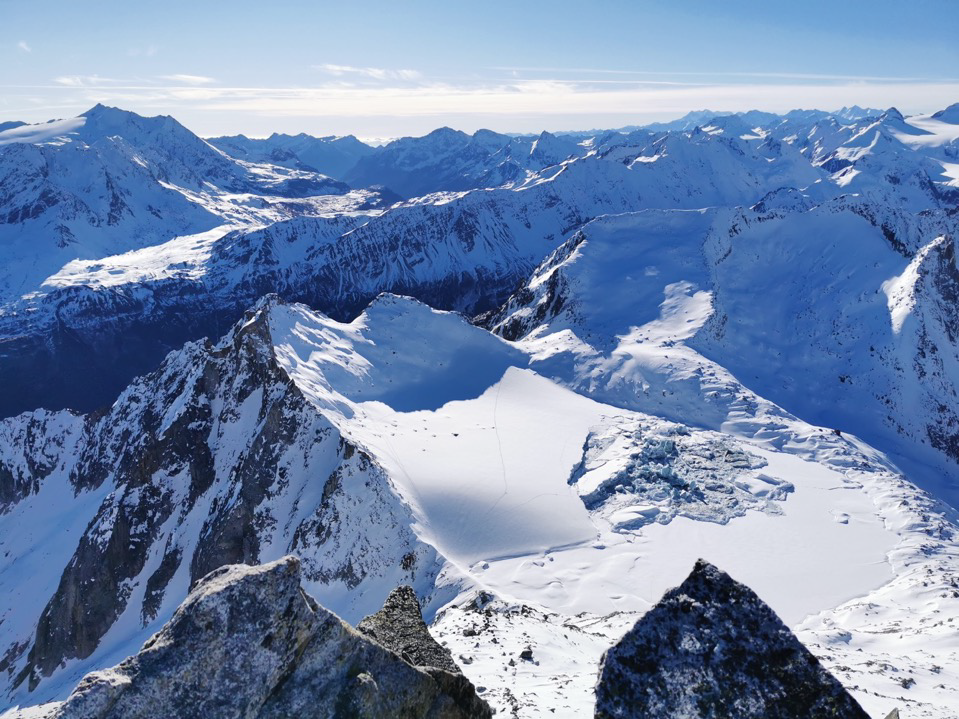
\includegraphics[width=0.5\textwidth]{\dir/Chueboden_picture.png}
\caption{Chüebodengletscher on 29.11.2021. Picture by Jasmine Vismara.}
\label{fig:photo}
\end{figure}


\section{Methods}

We aim to calculate the ice volume of Chüebodengletscher and to map the underlying bedrock. This is achieved by the following four steps. First, the glacier area and the glacier digital elevation model (DEM) are determined from aerial images. Second, the ice thickness is calculated from field observations using ground penetrating radar (GPR). In a third step, the GPR observations are interpolated over the glacier area using the GlaTE algorithm \citep{Langhammer&al2019}. Finally, the distributed thickness map obtained by GlaTE is subtracted from a DEM of the surface to obtain a map of the glacier bedrock topography. The following four sub-sections detail these four steps.

\subsection{Glacier outline and digital elevation model (DEM)}
\label{subsection:glacierarea}

The glacier outline (i.e. the glacier extent) was determined from ADS100 Image strips (ground sampling distance of $\sim$0.2\,m) from the Swiss Federal Office of Topography (swisstopo) acquired during flights commissioned by the Swiss Federal Office of the Environment on 9 September 2020\footnote{\url{https://api.geo.admin.ch/rest/services/luftbilder/MapServer/ch.swisstopo.lubis-bildstreifen/12501202009090750/extendedHtmlPopup?lang=en}}. The glacier area at that time was 0.12\,km$^2$. Note that the images were taken before the calving event. The DEM was derived from these images by swisstopo by using stereophotogrammetry, aerotriangulation, and ground control points (maximum resolution of 0.5\,m).

\subsection{Ice thickness from ground penetrating radar (GPR)}

GPR is a widely used geophysical method to scan the earth subsurface, in particular glacier subsurfaces. The GPR is constituted of a transmitter that sends a series of electromagnetic pulses at high frequency through antennas. These pulses are scattered when they encounter a change in physical properties, and are eventually reflected back to the GPR receiver (Fig.~\ref{fig:gpr}). The physical properties of interest are permittivity and conductivity. Because the permittivity and conductivity contrast between ice and rock is large, this allows the ice-bedrock interface at the bottom of the glacier to be detected. The travel time of the reflected pulse between the surface and the bedrock is recorded by the GPR, and is converted into distance by knowing the pulse velocity in the ice. 

\begin{figure}
\centering
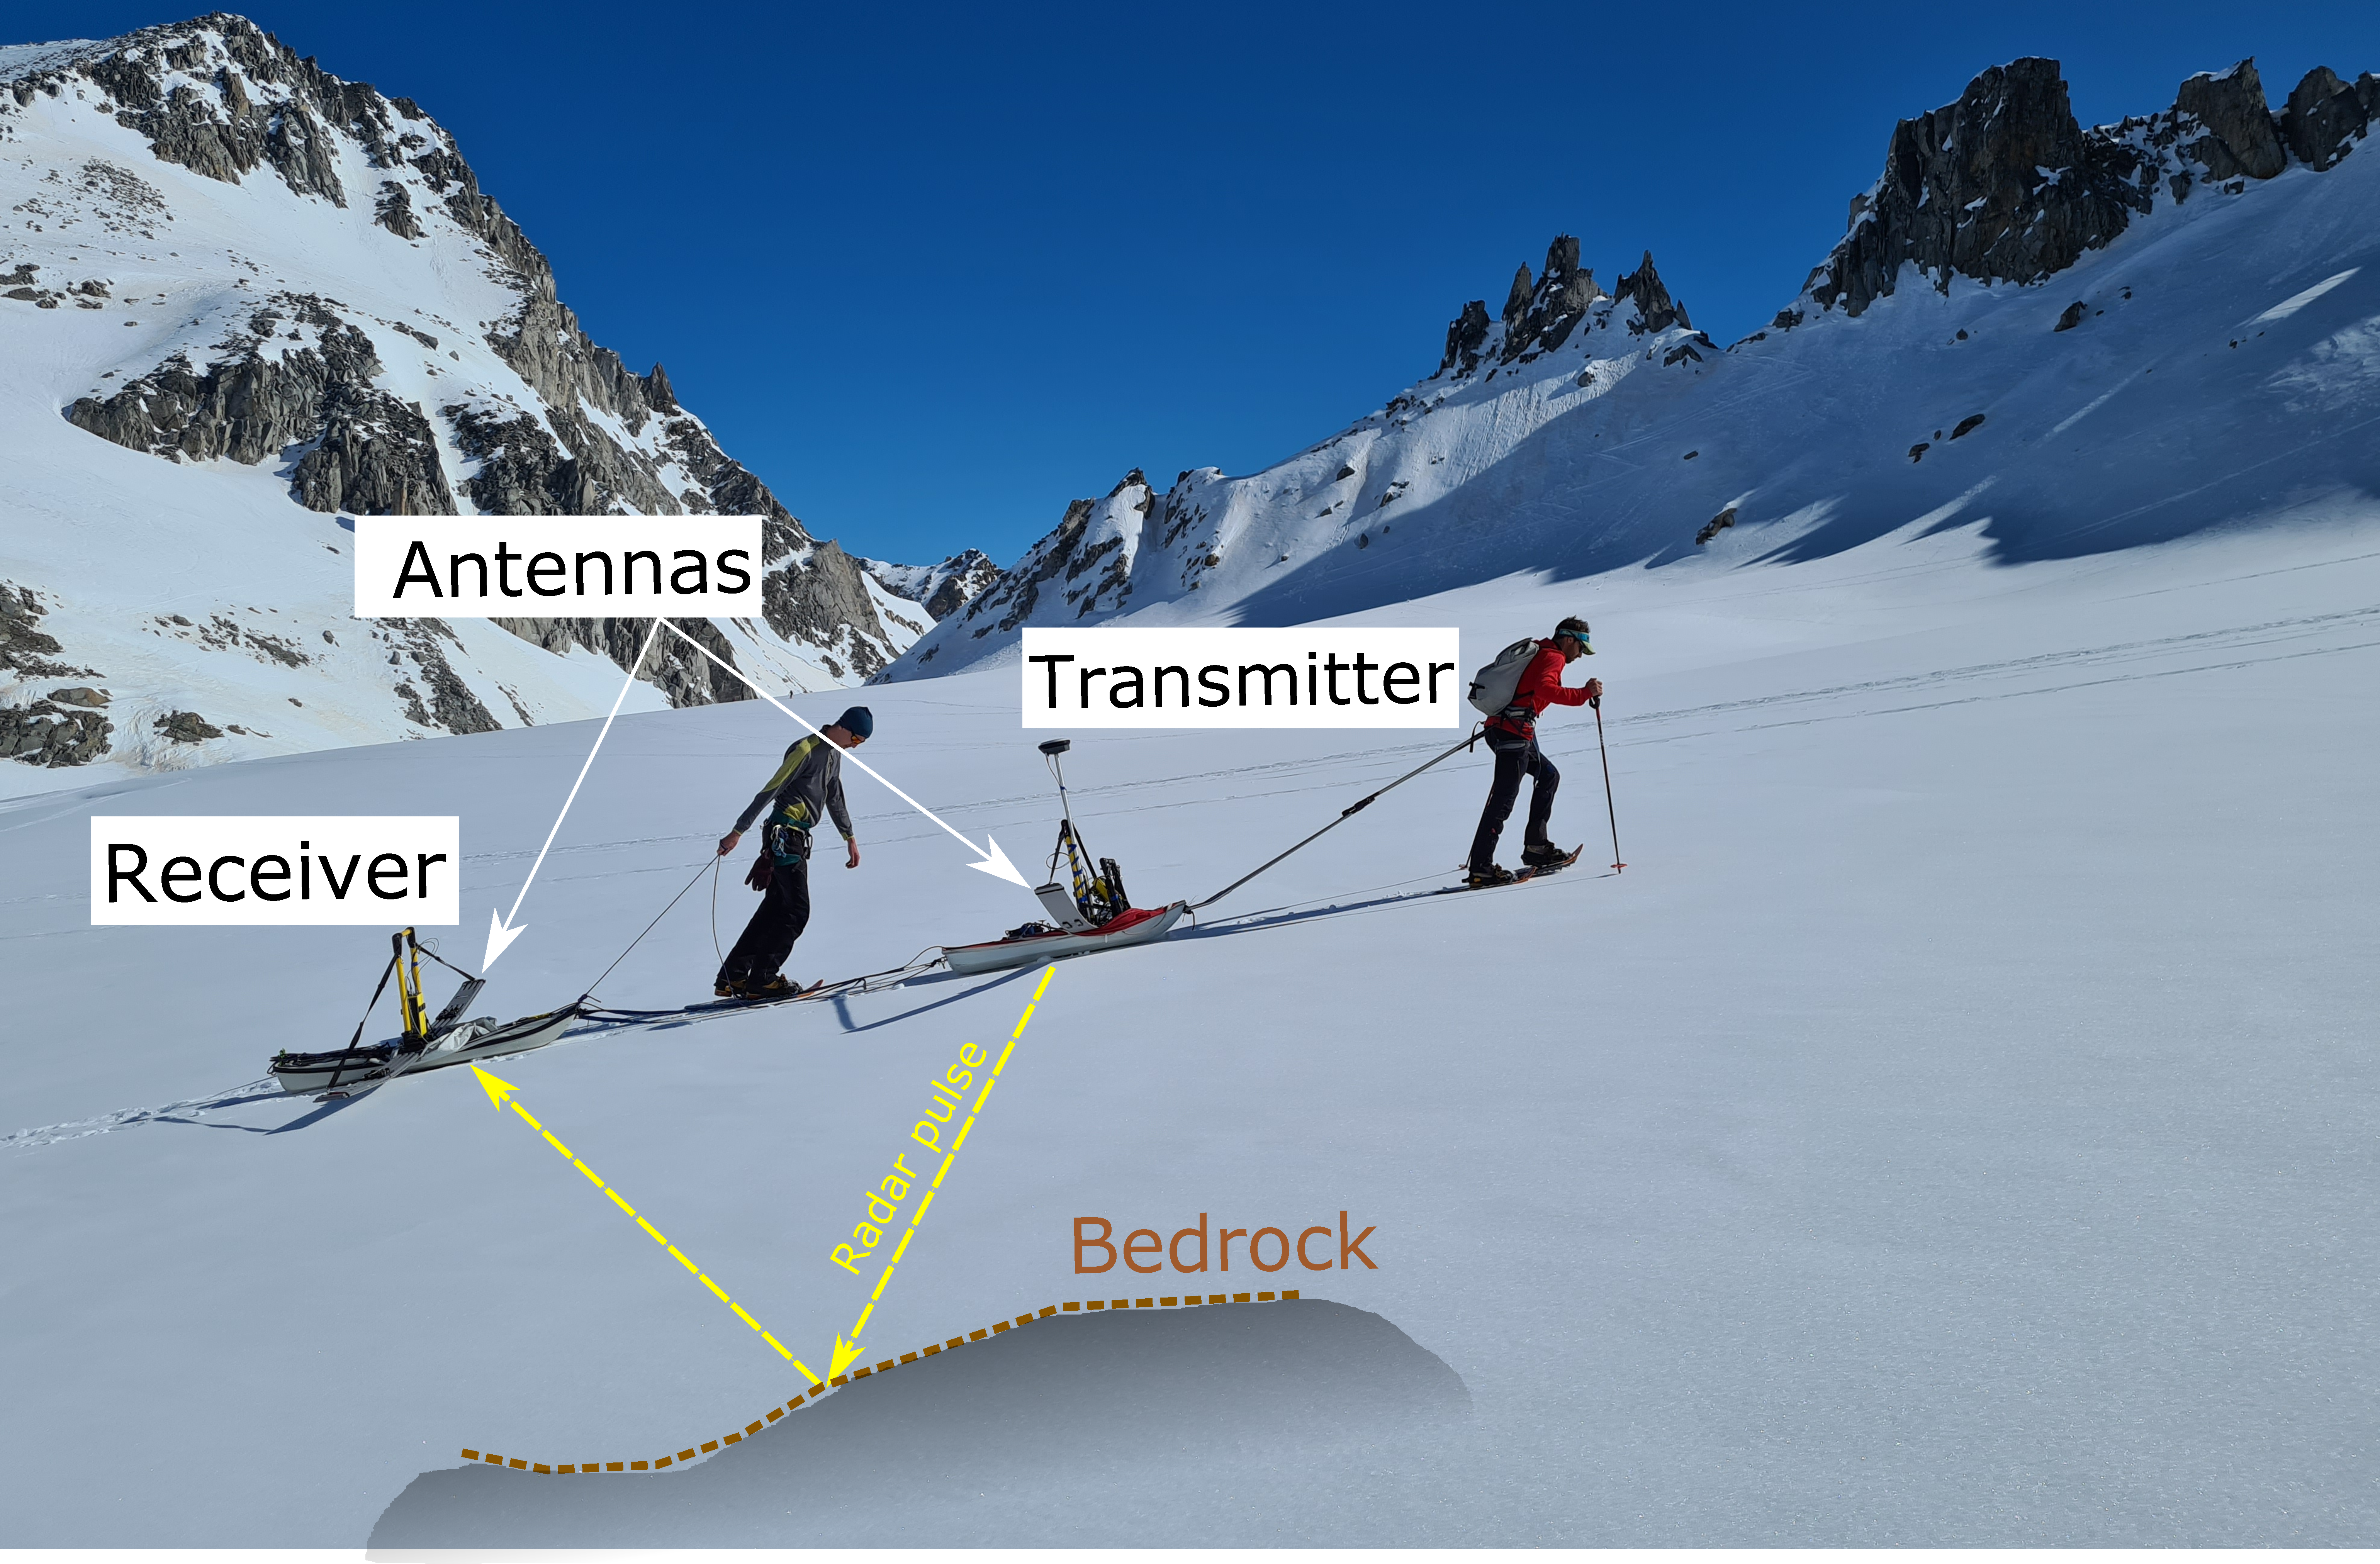
\includegraphics[width=0.8\textwidth]{\dir/gpr_chueboden.pdf}
\caption{GPR system during the ice thickness field measurements at Chuebodengletscher.}
\label{fig:gpr}
\end{figure}

The GPR field campaign took place on 31 March 2021. The GPR was mounted on two sledges (Fig.~\ref{fig:gpr}). Seven GPR lines were performed, both perpendicular and parallel to the glacier flow (Fig.~\ref{fig:fig1}). Note that twelves lines were initially conducted, but five of them failed due to either battery or global navigation satellite system (GNSS) issues in the field. The characteristics of the GPR survey are presented in Table~\ref{tab_gpr}. The data were processed with an in-house MATLAB-based toolbox \citep[e.g.][]{Langhammer&al2019}. The processing steps to obtain the ice thickness are detailed in Table~\ref{tab:processingflowGPR}. For the ice thickness calculation, we uniformly subtracted the snow depth from the surface elevation. This is motivated by snow depth measurements performed at three different places, which all showed similar snow-depth values (4\,m, see Section~\ref{section:codeanddata} for details). Note that the vertical accuracy of the GPS position was only $\pm$\,5\,m because of a failure in the GNSS that day. 

\begin{figure}[h!]
\centering
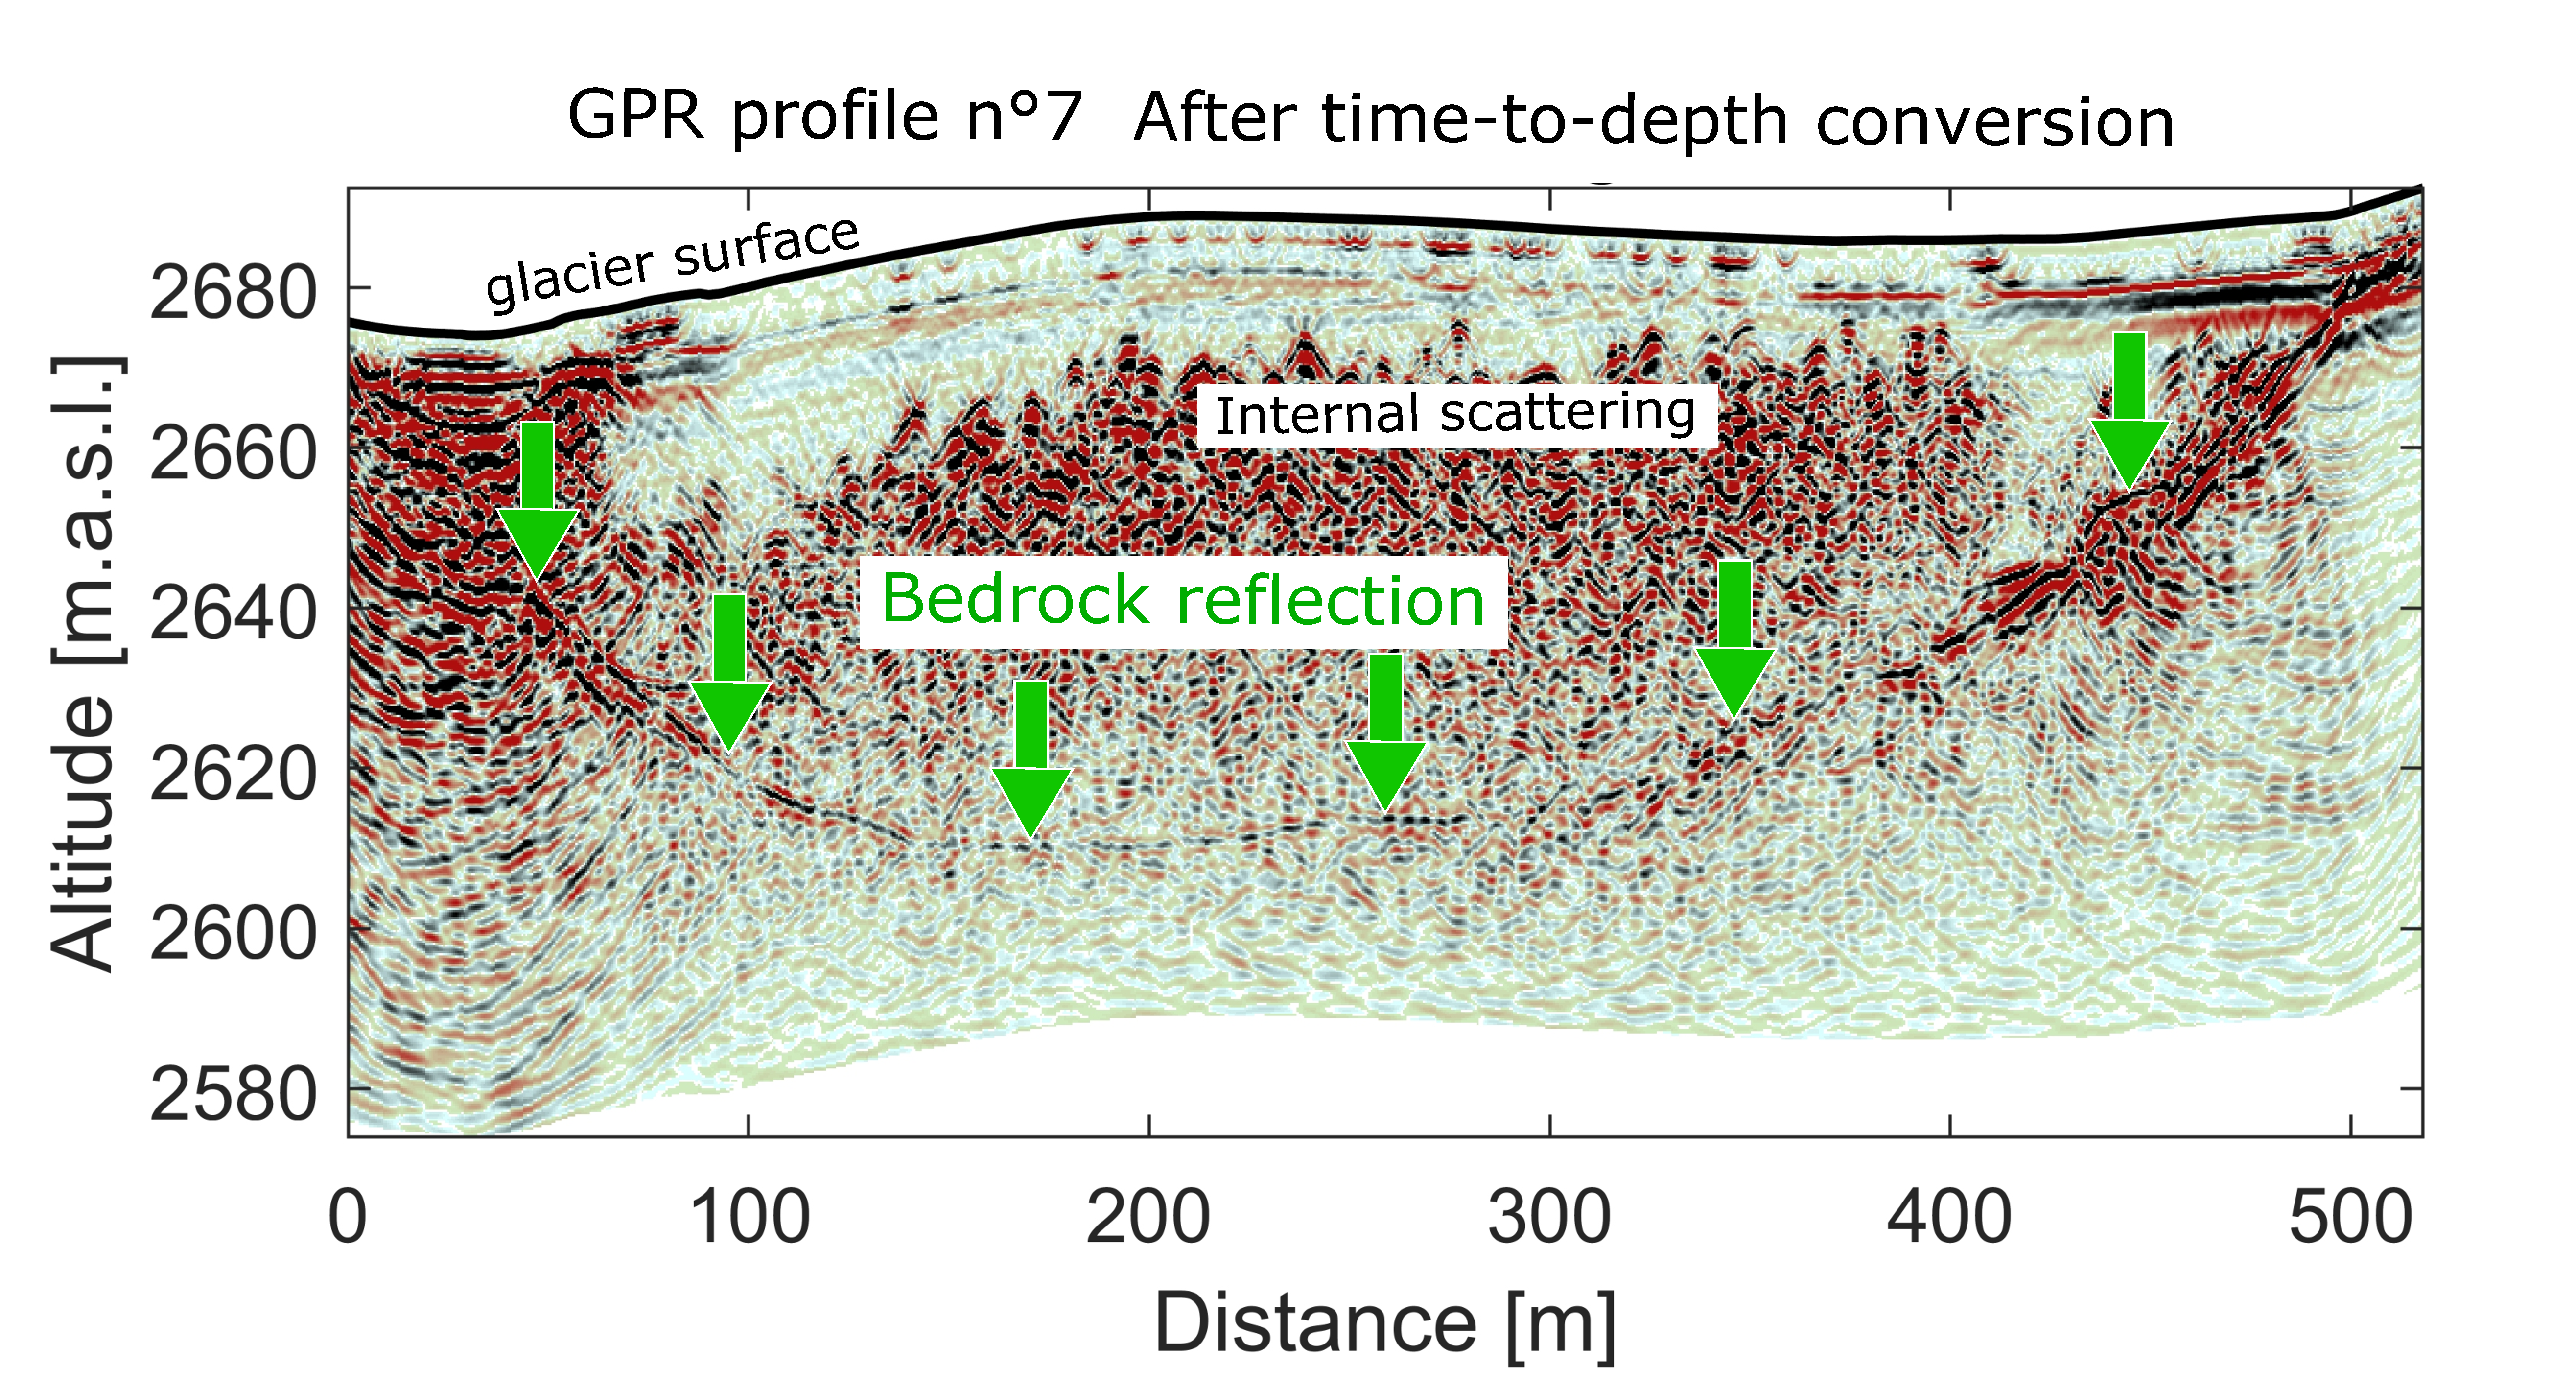
\includegraphics[width=0.8\textwidth]{\dir/profile7.pdf}
\caption{Example of picking bedrock in a radar section to determine ice thickness.}
\label{fig:prof7}
\end{figure}

\begin{figure}[h!]
\centering
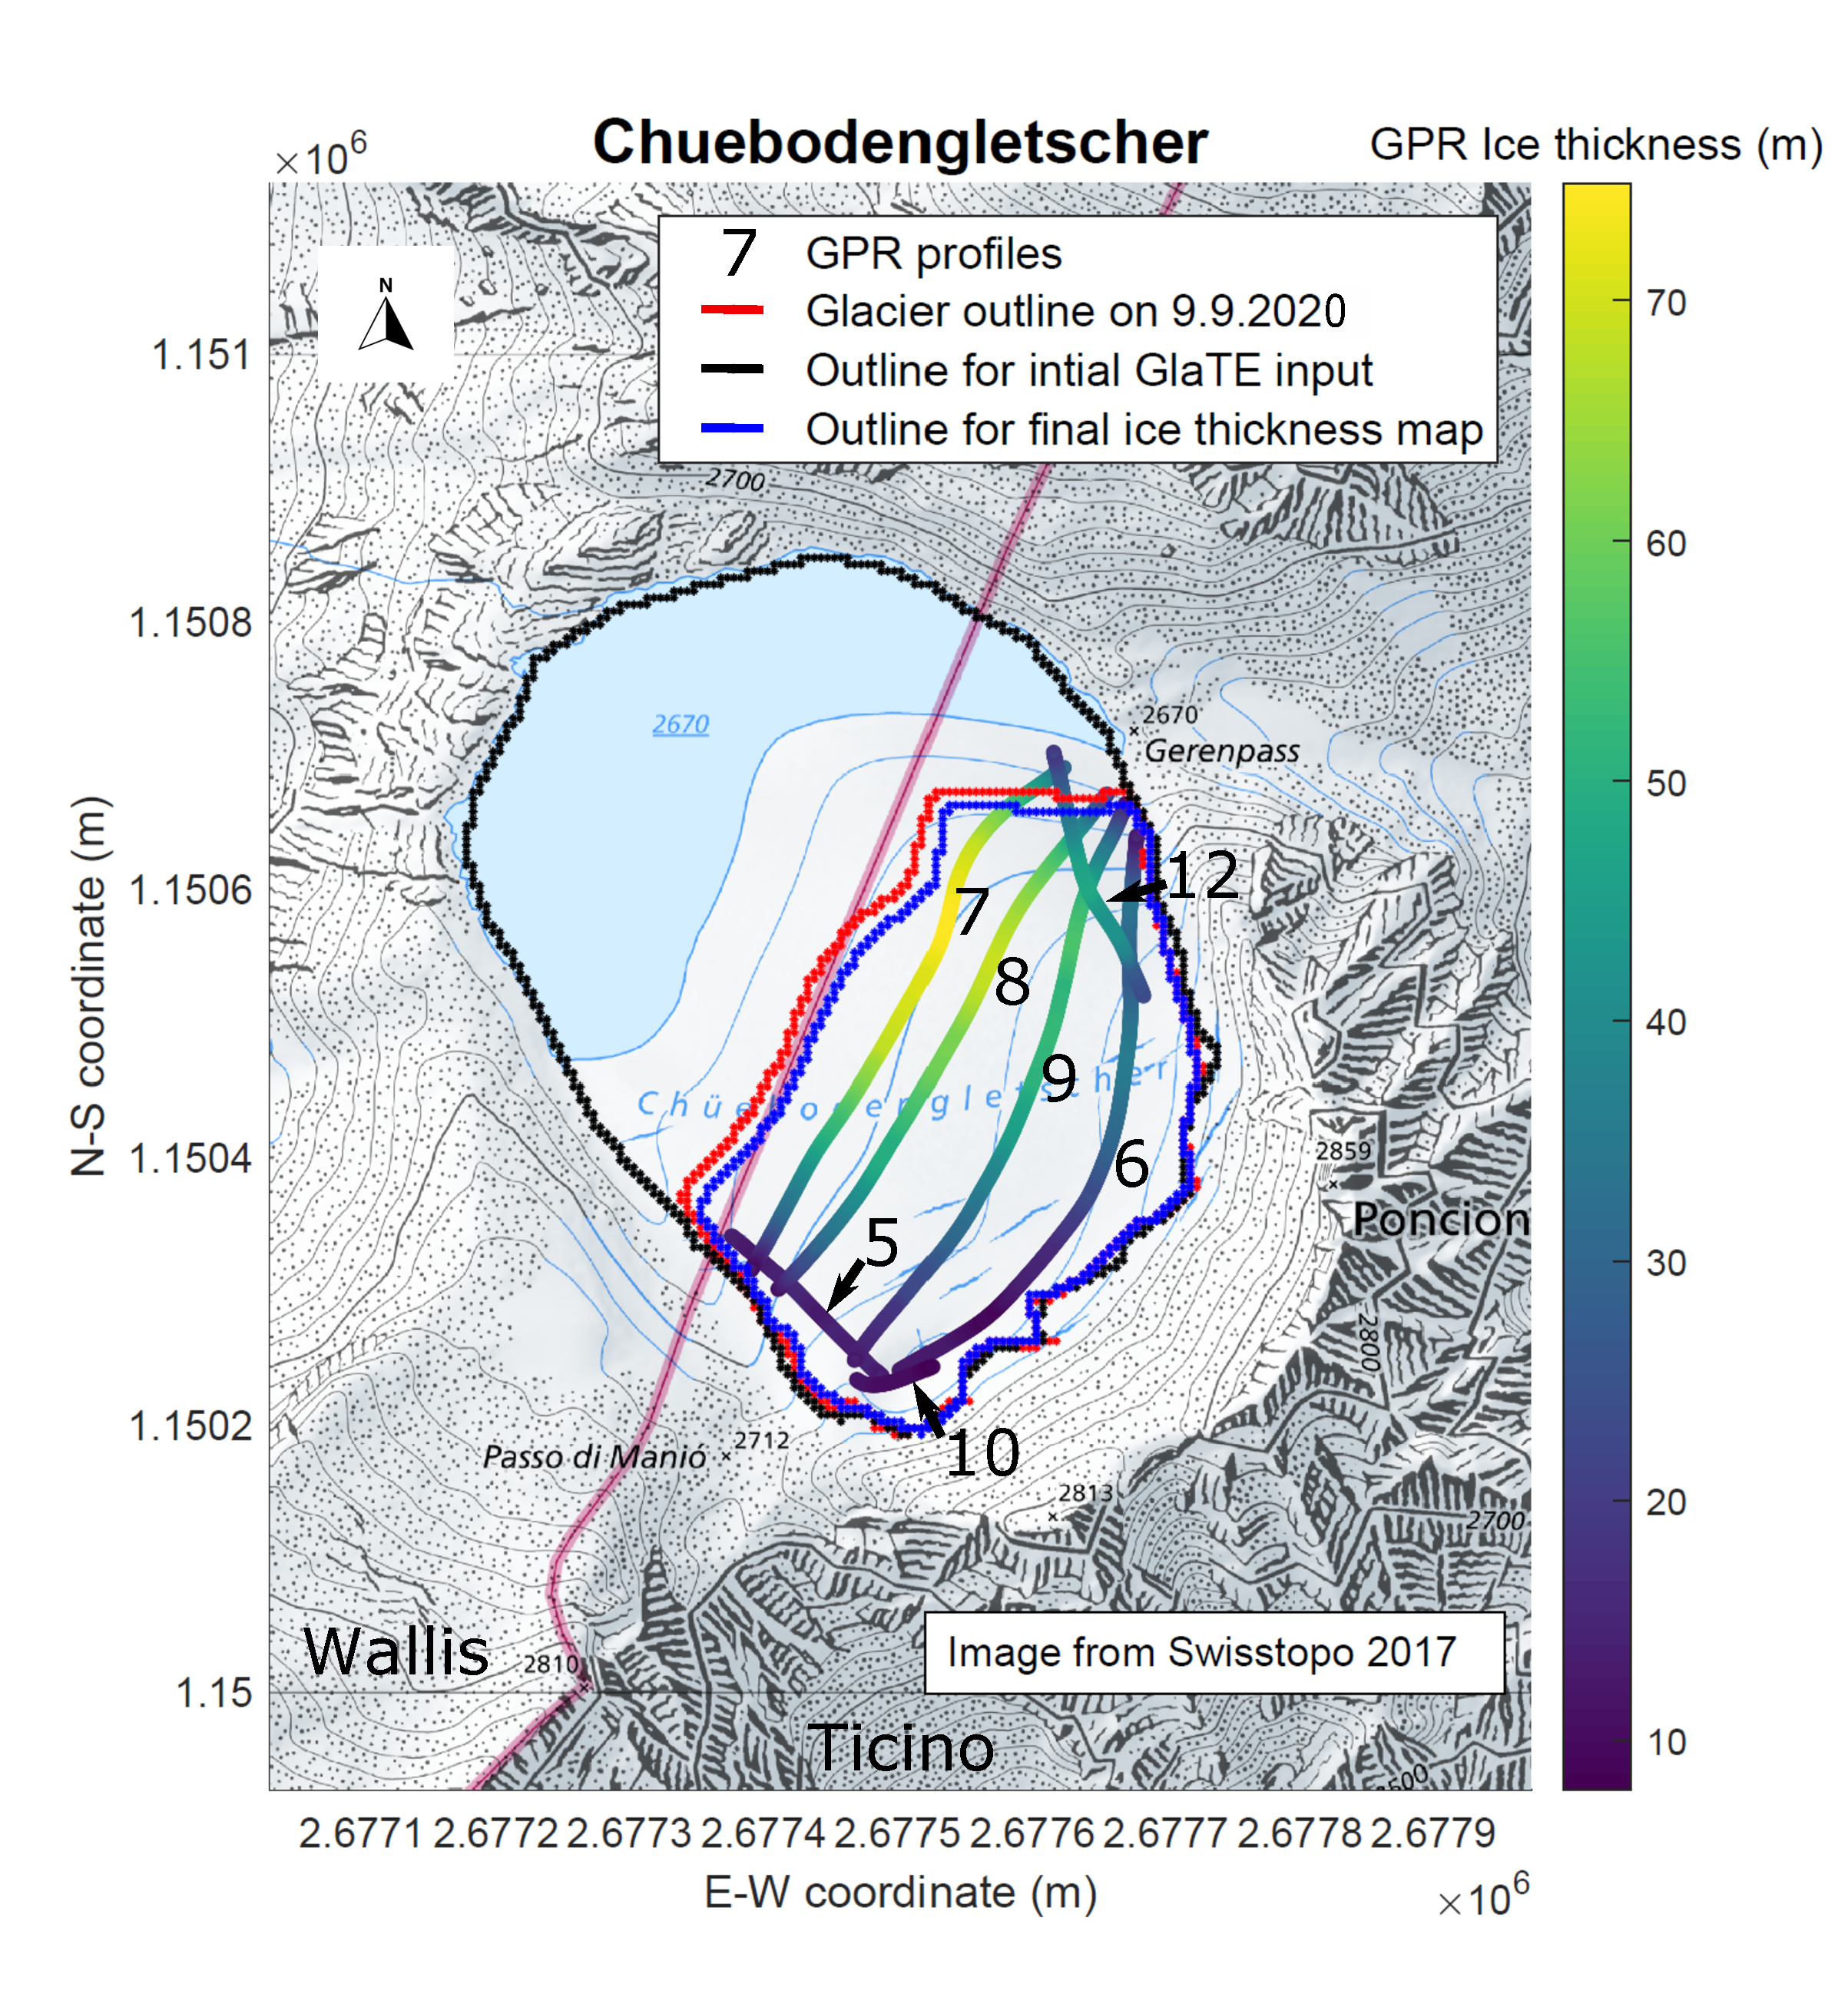
\includegraphics[width=0.9\textwidth]{\dir/Fig1.pdf}
\caption{Point-scale ice thickness measurements along the seven GPR profiles. The distributed ice thickness map is computed within the blue outline. The blue outline represents 92\,\% of the total glacier area in September 2020. The latter is marked by the red outline.}
\label{fig:fig1}
\end{figure}

\begin{table}[h!]
    \centering
    \begin{tabular}{l c r}
         \hline
\textbf{GPR parameters}  & \textbf{Value} & \textbf{Remarks} \\
\hline
Frequency & 25 MHz  \\
Sampling interval & 0.4 ns \\
Time window & 2640 ns / 440 m & two way traveltime\\
Antenna separation & 4 m \\
Antenna step size & 1 m \\
Radar velocity in ice & 0.167 m\,ns$^{-1}$ & value by default \\
System Stacking & 8 & \\
GPS input & Internal GPS & precision $\pm$5\,m\\
\hline
    \end{tabular}
    \caption{GPR parameters for Chüebodengletscher survey.}
    \label{tab_gpr}
\end{table}


\begin{table}[h!]
    \begin{center}
    \begin{tabular}{l l l}
        \hline
         \textbf{} & \textbf{Processing step} & \textbf{Comments} \\
         \hline 
         1. & Smooth GPS profile & Moving average of coordinates over 500 traces\\
         2. & Set time zero and record length & 2640\,ns ($\approx$ 220\,m depth penetration in ice)\\
         3. & Background noise removal &\\
         4. & Trace binning along profile & Binned to 0.5\,m spacing\\
         5. & Butterworth bandpass filter & 10-75\,MHz\\
         6. & Kirchoff migration &\\
         7. & Time-to-depth conversion & Constant velocity 0.167 m\,s$^{-1}$\\
         8. & Bedrock elevation picking & Manually (see Figure~\ref{fig:prof7})\\
         9. & Ice thickness calculation & Uniform snow depth = 4\,m\\
         \hline
    \end{tabular}
    \caption{Overview of the processing flow for the GPR data}
    \label{tab:processingflowGPR}
    \end{center}
\end{table}



\subsection{Ice thickness interpolation at the glacier scale}
\label{subsection:glate}

The ice thickness obtained from the GPR profiles was interpolated by using the glacier thickness estimation algorithm ``GlaTE'' \citep{Langhammer&al2019}. GlaTE obtains the distributed ice thickness of a glacier by optimally combining modelling results (glaciological constrain) and measured ice thickness (GPR data). The GlaTE inputs are: a glacier outline, a glacier surface DEM, and possibly observational data (e.g. GPR measurements). The algorithm had been used to estimate the ice thickness of Chüebodengletscher before \citep{Grab&al2021}, but the existing results were obtained without GPR data, thus making them less reliable. The DEM obtained in Section~\ref{subsection:glacierarea} was re-sampled to 5\,m to reduce the computational cost and to avoid non-physical interpretations of the results between the GPR lines. In contrast to most alpine glaciers, Chüebodengletscher has a non-zero ice thickness at one of its borders, i.e. at the calving front. Because GlaTE was not designed for such glaciers, we implemented a slight modification in the original procedures. First, we ran GlaTE over the glacier and lake area (black outline in Fig.~\ref{fig:fig1}) assuming zero ice thickness at the borders. Since the boundary of the interpolation is far away from the calving front, the procedure avoids the front being affected by the zero ice thickness conditions. The influence of the out-of-glacier topography was not taken into account ($\lambda_2$=0 in Appendix A of \cite{Grab&al2021}). In a second step, we applied the glacier mask (blue outline in Fig.~\ref{fig:fig1}) to artificially cut the ice thickness at the calving front. Note that this new mask is ca. 15\,m inward the glacier at the calving front, and that the new mask represents ca. 92\,\% of the total glacier area. We applied this inward-cut to minimize the strong gradient at the glacier-lake transition. These two steps respect the zero ice thickness at the ground-based glacier border, and allow for a calving front at the lake-terminating glacier border. The ice volume is finally obtained by integrating the distributed ice thickness over the glacier area.  


\subsection{Glacier bedrock elevation}
\label{subsection:bedrock}

The bedrock elevation under the glacier was calculating by subtracting the distributed ice thickness obtained by GlaTE (see Section~\ref{subsection:glate}) from the glacier surface elevation obtained by the 2020 DEM (see Section~\ref{subsection:glacierarea}). 


\section{Results}

\subsection{Ice thickness}

Figure~\ref{fig:fig2}a presents the ice thickness of Chuebodengletscher as obtained from linear interpolation of the GPR measurements, whilst Figure~\ref{fig:fig2}b shows the ice thickness as interpolated by using GlaTE. Both grids have a resolution of 5\,m. We found a maximal ice thickness of 75\,m, which is ~40\,m deeper than the previous estimation by \citet{Grab&al2021}. During the field campaign, a GPR profile was acquired close to the calving front. However, due to GPS failure, this profile couldn't be placed accurately on the map. Consequently, we did not consider this profile in our calculations. This notwithstanding, the radar section associated to this profile show a maximal depth of 78\,m, in line with the 75\,m ice thickness calculated close to the calving front.

\begin{figure}[h!]
\centering
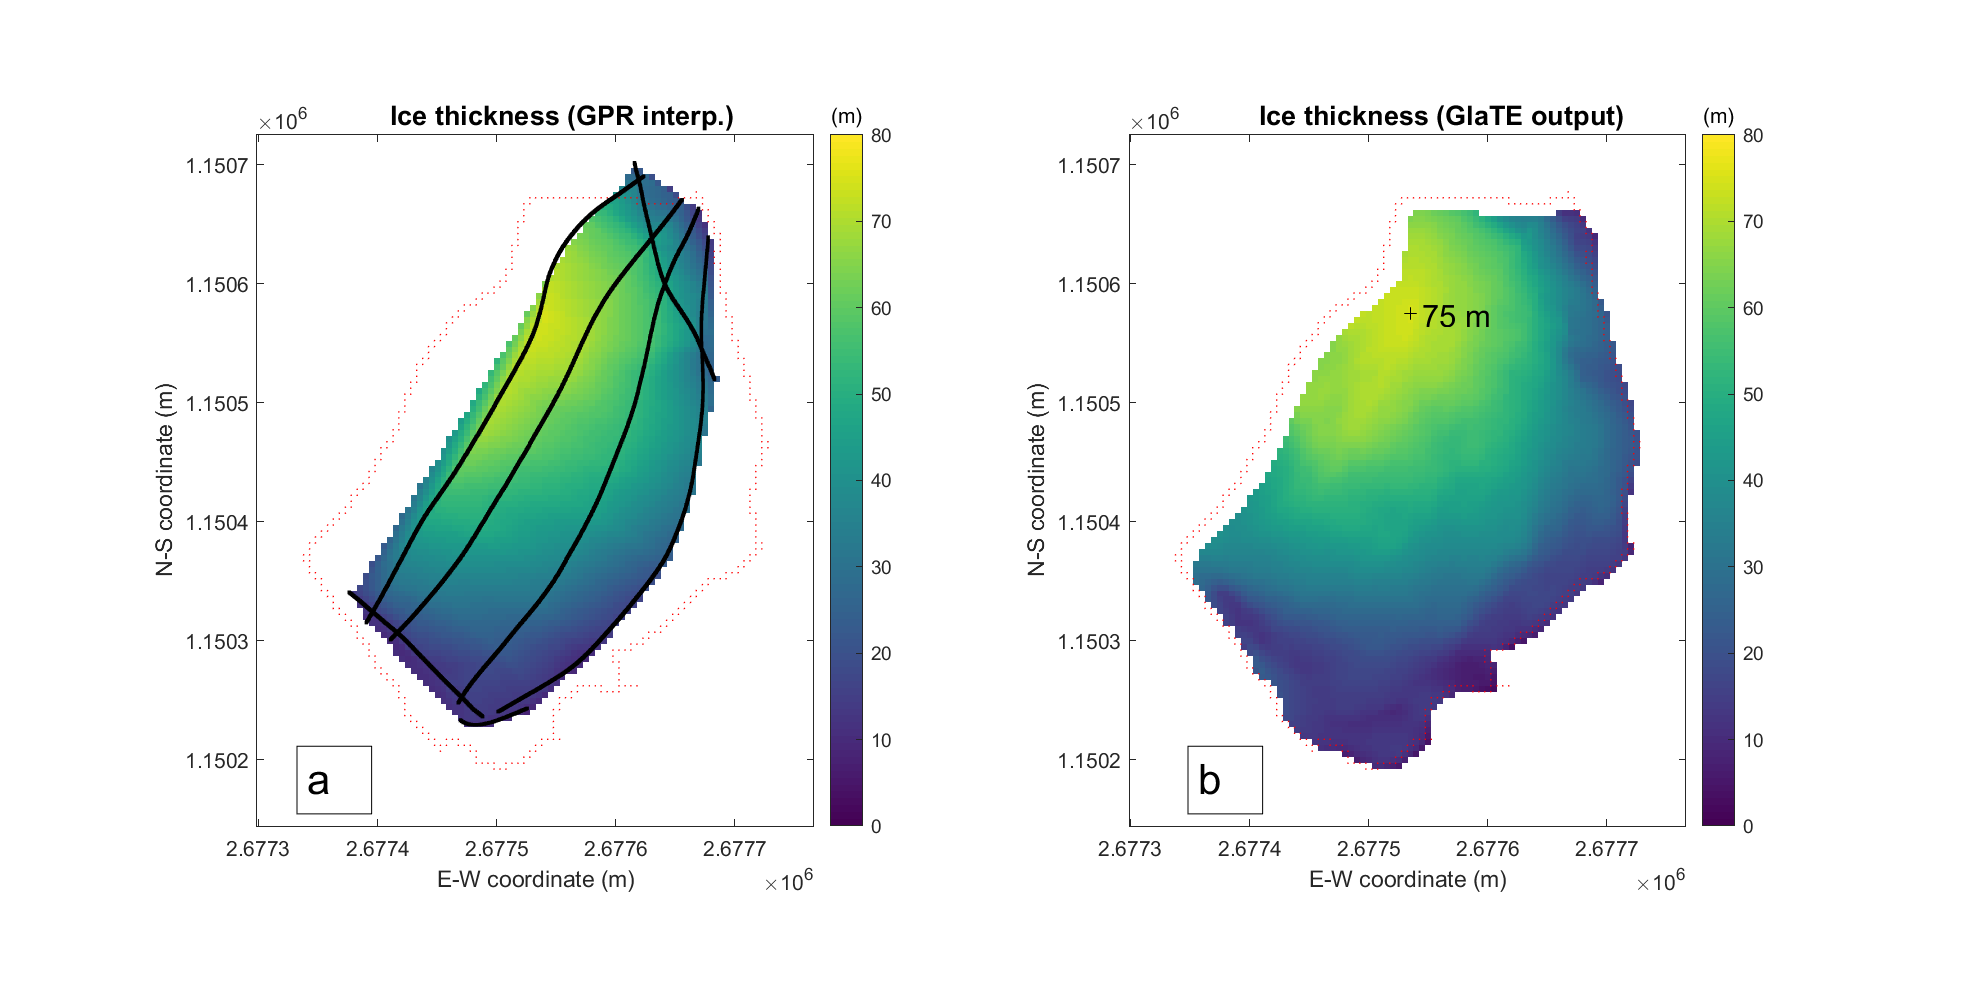
\includegraphics[width=1\textwidth]{\dir/Fig2.png}
\caption{a) Linear interpolation of GPR ice thickness measurements. GPR profiles are represented by the black lines. b) Ice thickness interpolation as obtained by GlaTE when using both GPR and glaciological constrain. The thickest ice (75m) is marked by the cross. Glacier outline on September 2020 (before calving event) is indicated in red. The grid resolution is 5\,m.}
\label{fig:fig2}
\end{figure}

\subsection{Glacier bedrock elevation and lake bathymetry}


Figure~\ref{fig:fig3} presents the glacier bedrock elevation as calculated in Section~\ref{subsection:bedrock}. Additionally, Figure~\ref{fig:fig3}a presents the lake depth measurements conducted by Giovanni Kappenberger on 15.10.2021 (see Section~\ref{section:codeanddata} for raw data). These values are in line with our bedrock map and suggest that the maximal lake depth is close to the current glacier front, at ca. 2710\,m a.s.l. 

\begin{figure}[h!]
\centering
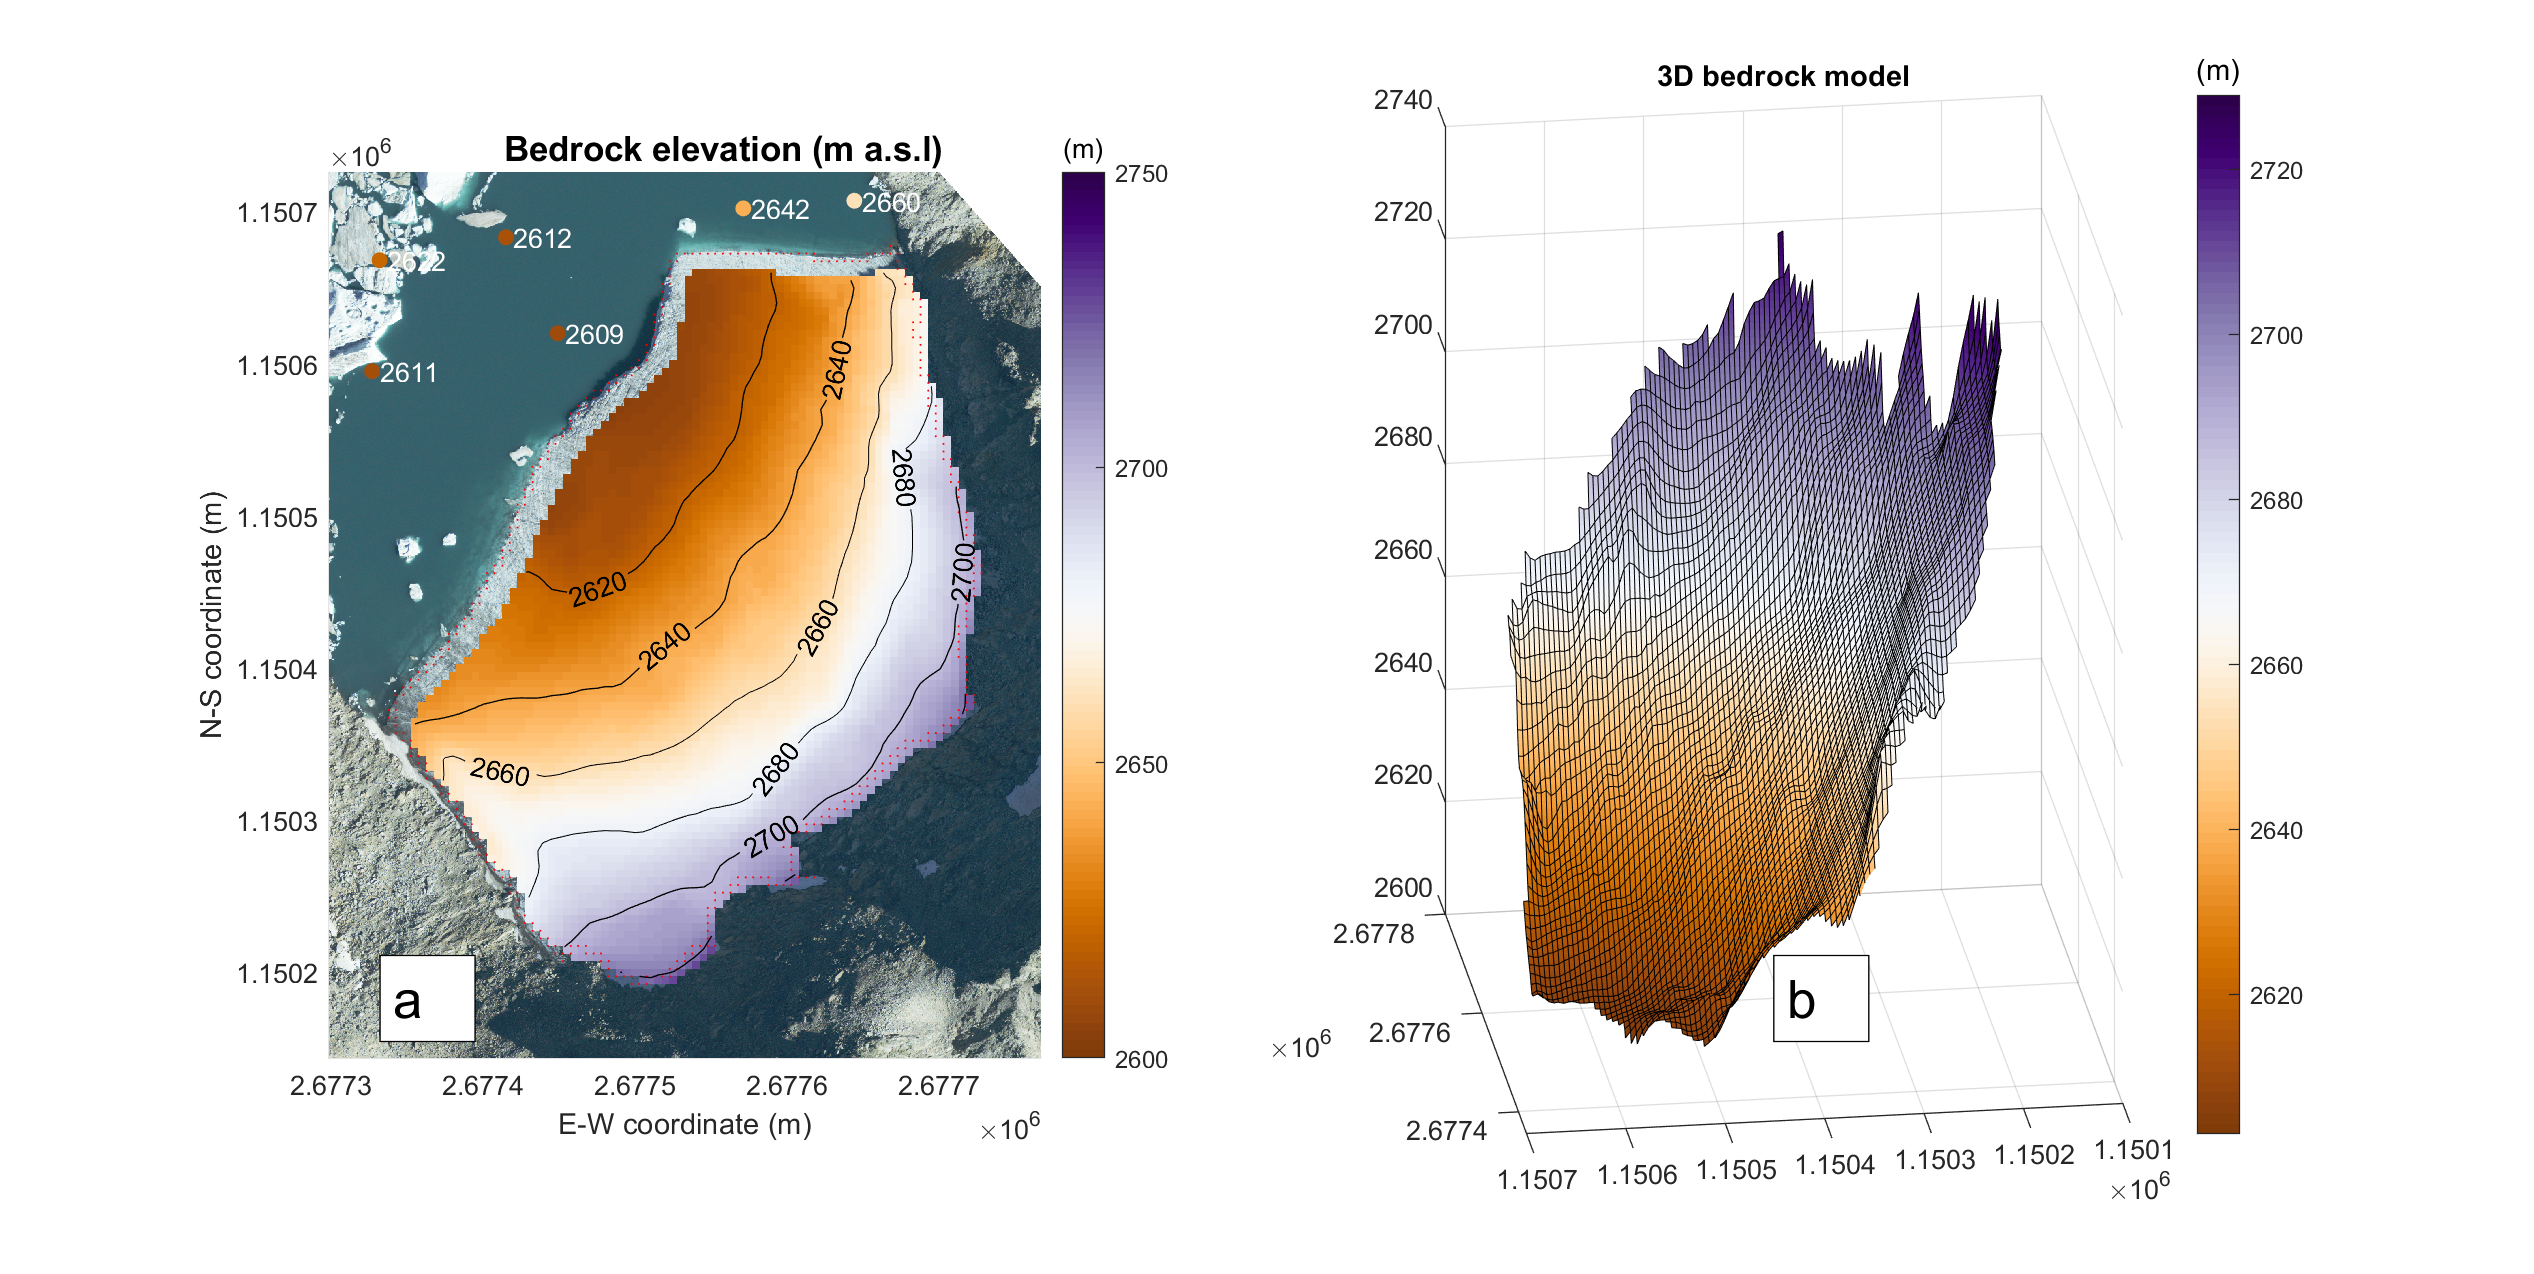
\includegraphics[width=1\textwidth]{\dir/Fig3.png}
\caption{a) Glacier bedrock elevation derived from the ice thickness. The dots represents additional lake bathymetry points-measurements performed by Giovanni Kappenberger on 15.10.2021. The background photo was taken on 9 September 2020 by the Swiss Federal Office of Topography. b) 3D visualization of the glacier bedrock. Note that the vertical axis is exaggerated for better visibility. The grid resolution is 5\,m in both plot.}
\label{fig:fig3}
\end{figure}

\subsection{Ice volume}

We calculated an ice volume of 4.35\,$\times$\,10$^6$\,m$^3$ for the 92\,\% of the glacier area on September 2021. Note that the 8\,\% of the missing area corresponds to 0.01\,km$^2$ located at the calving front, where ice is the thickest. The corresponding ice volume missing at this date is thus more that 8\,\% of the total volume. The calculations are done by considering the glacier prior to the calving event. By consequence, the actual, present-day volume is smaller. The volume of the ice detachment that occurred in November 2021 can be estimated by integrating the calculated ice thickness over the calved area. For this, an outline of the calved area would be necessary. We expect this to become available when the 2021-image acquired by the Swiss Federal Office of Topography will be released (presumably in early 2023). An alternative would be to obtain such an outline from a orthoimage acquired on site, e.g. through a dedicated UAV survey.  

\subsection{Uncertainties and limitations}

The point-specific uncertainty in bedrock elevations includes uncertainties from (i) the GlaTE ice thickness interpolation, (ii) the GPR data ($\pm$\,5\,m), and (iii) the elevations of the surface DEM ($\pm$\,2\,m). Although "ii" and "iii" are known, we didn't evaluate the uncertainties for each grid cells of the glacier. The ice volume uncertainty is expected to be substantially smaller than the point-specific uncertainty described above, since random uncertainties of neighbouring pixel cancel out each other when integrating over the glacier extent. For further considerations of uncertainties estimation, see Section 4 and Appendix D in \cite{Grab&al2021}.

Future users of the presented thickness and bedrock map have to be aware of several limitations. First, GlaTE is known to slightly overestimate the bedrock slope close to the glacier borders \citep{Grab&al2021}. This is also the case here. This results in overestimated ice thickness close to the borders. Second, some location of the glacier have inaccurate ice thickness because of the distribution of GPR profiles, and because of modelling constrains. For instance, the glacier left hand side (bottom left at Fig.~\ref{fig:fig3}a) show a suspicious topographic dorsal (``ridge'') at the bedrock surface. This can be seen on the color contrast at the bottom left in Fig.~\ref{fig:fig2}b, on the contour lines at the bottom left in Fig.~\ref{fig:fig3}a, and at the right side of Fig.~\ref{fig:fig3}a. This is due to the disagreement between the GlaTE algorithm (ice thickness overestimation close to the border) and GPR-profile nr 5. Although local ice thickness estimation can suffer of such anomalies, we believe that the overall thickness is well constrained by the GPR observations and the model. 


\section{Data and Code availability}
\label{section:codeanddata}

The data and the code necessary to obtain the ice thickness and the bedrock elevation are available from ETH's Research Collection under the following DOI: \href{https://doi.org/10.3929/ethz-b-000516258}{10.3929/ethz-b-000516258}. The material provided at the link allow for reproducing all results and figures contained within this report. Figure~\ref{fig:folder_three} presents the repository structure.


\begin{figure}[h!]
\centering
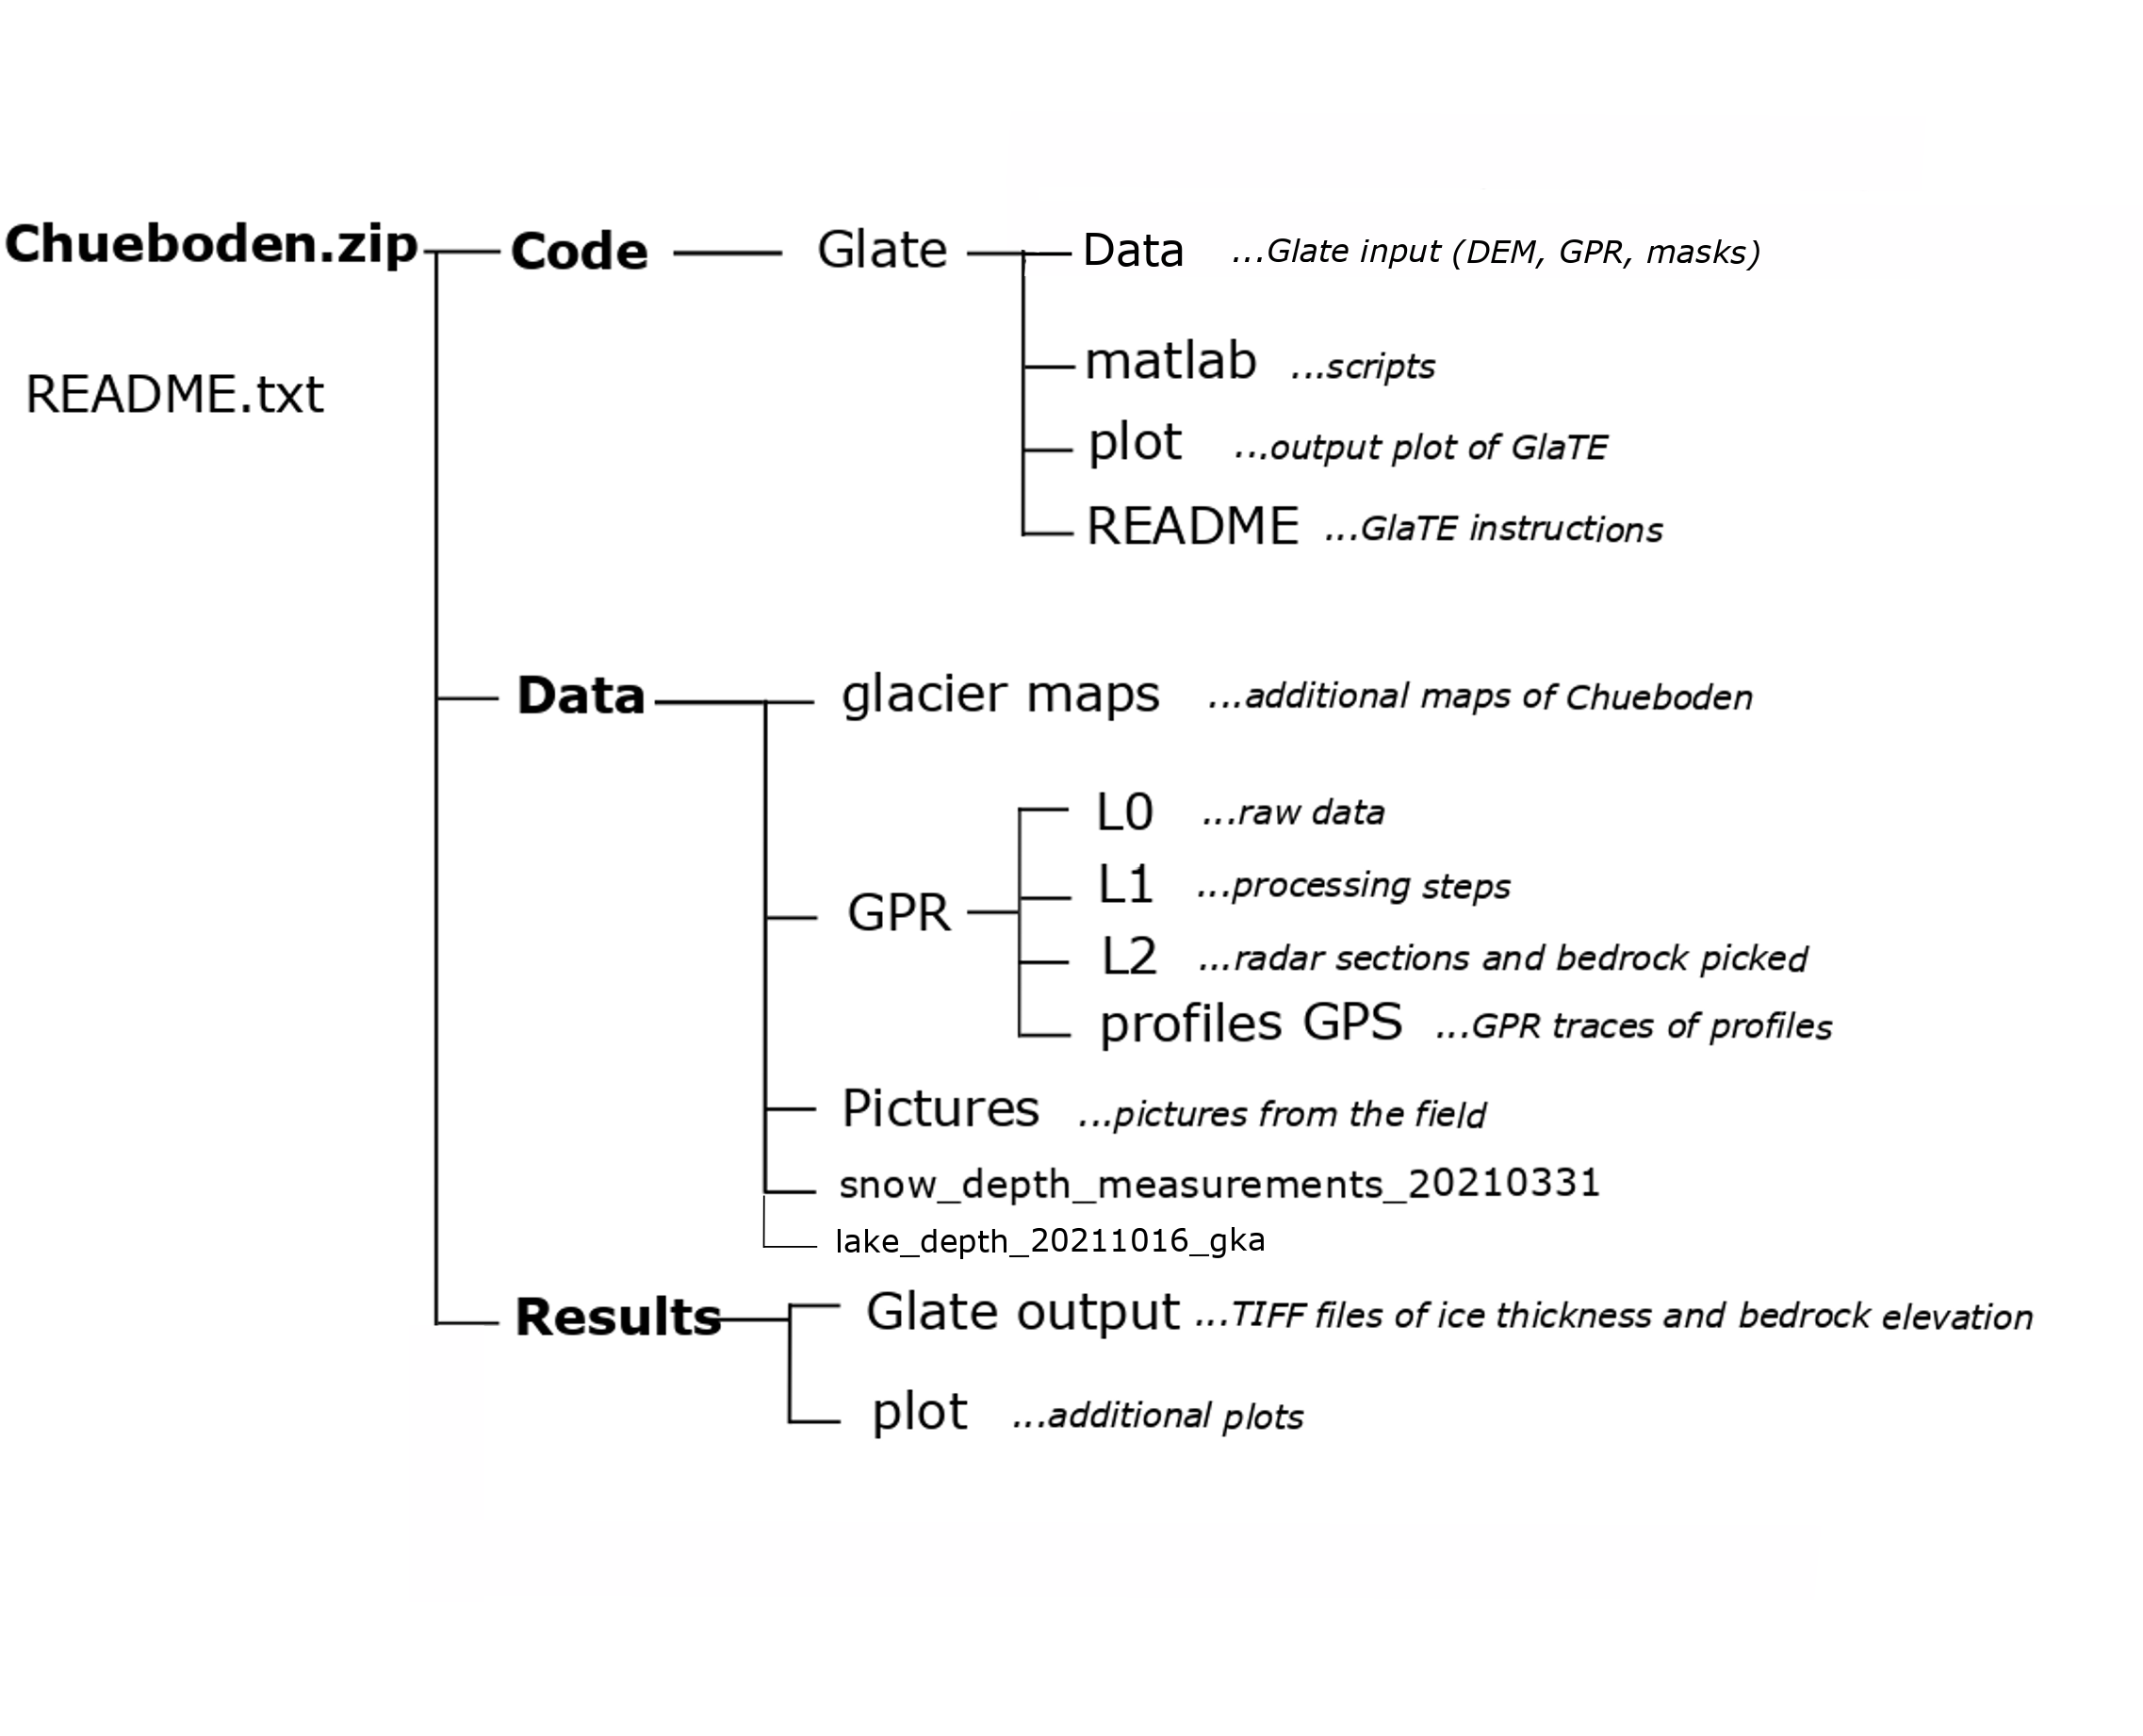
\includegraphics[width=0.75\textwidth]{\dir/folder_three.png}
\caption{Folder tree of the data repository available from ETH's Research Collection. The data can be accessed through the following DOI: \href{https://doi.org/10.3929/ethz-b-000516258}{10.3929/ethz-b-000516258}.}
\label{fig:folder_three}
\end{figure}

%\chapter[The hypothetical drainage of a water pocket]{Supplementary materiel for Chapter~\ref{ch:discussion}: The hypothetical drainage of the water pocket at Rhonegletscher in 2022}







